%!TEX root = ../paper.tex

% Small differences in anisotropy  
In \cref{s:results} some differences in anisotropy of the kernels were observed, however these differences were relatively small. This section investigates the anisotropy of the kernels. 
	
		% Single Sphere
		\begin{figure}
			\centering
			\begin{subfigure}{0.23\textwidth}
				\centering
				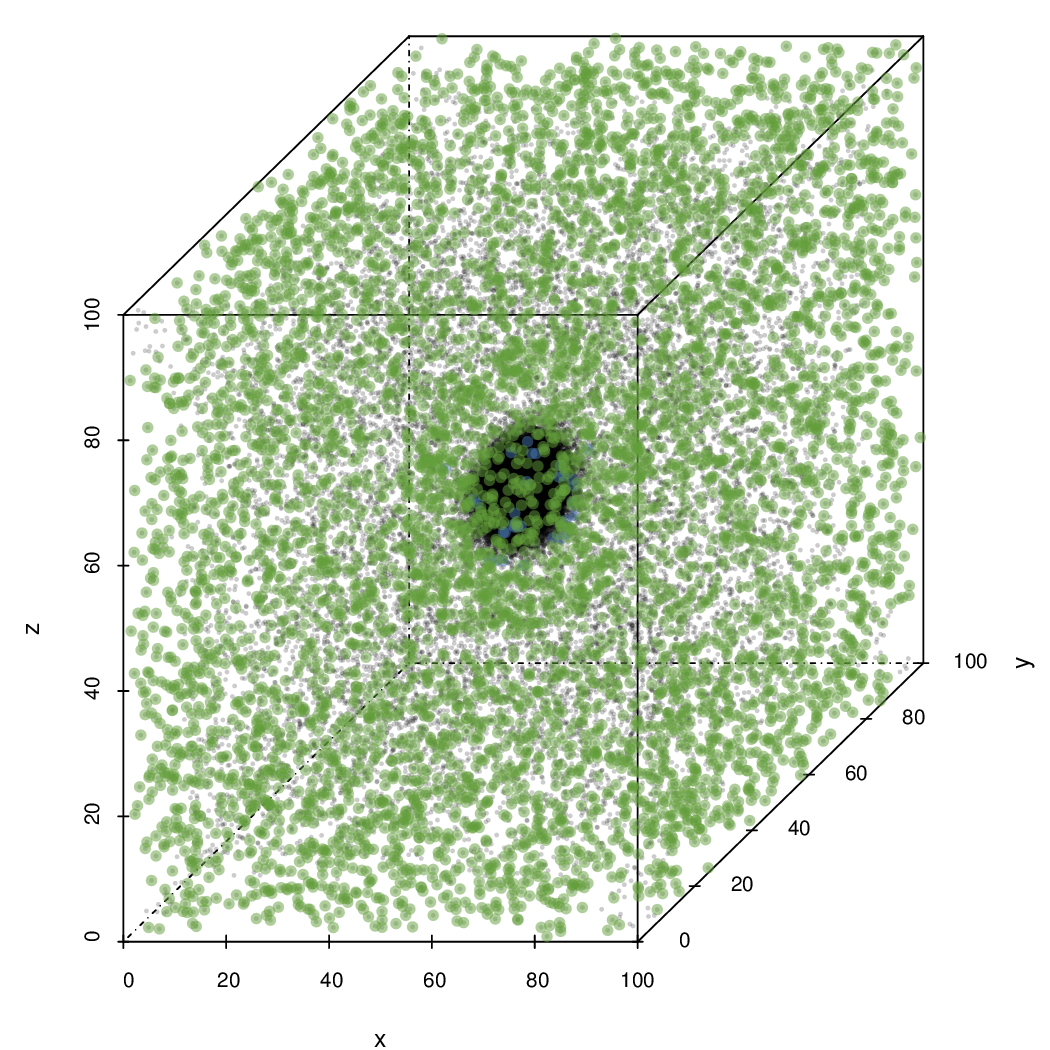
\includegraphics[keepaspectratio=true, width=\textwidth, height=0.23\textheight]{discussion/img/ferdosi_1_60000_anisotropy.png}
				\caption{Dataset \ferdosiOne}
				\label{fig:discussion:anisotropy:ferdosi1}
			\end{subfigure}
			\begin{subfigure}{0.23\textwidth}
				\centering
				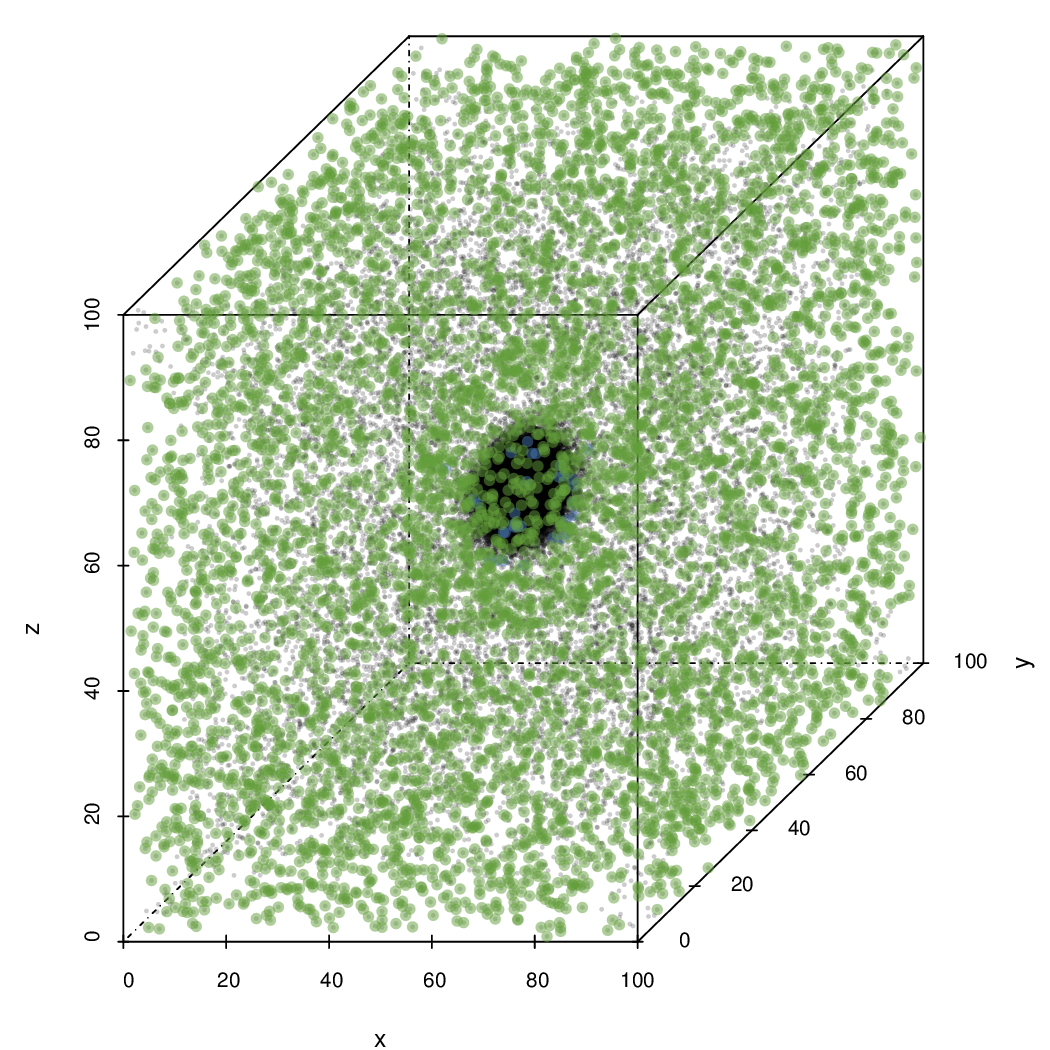
\includegraphics[keepaspectratio=true, width=\textwidth, height=0.23\textheight]{discussion/img/ferdosi_1_60000_anisotropy.png}
				\caption{Dataset \baakmanOne}
				\label{fig:discussion:anisotropy:baakman1}
			\end{subfigure}	
			\begin{subfigure}{0.23\textwidth}
				\centering
				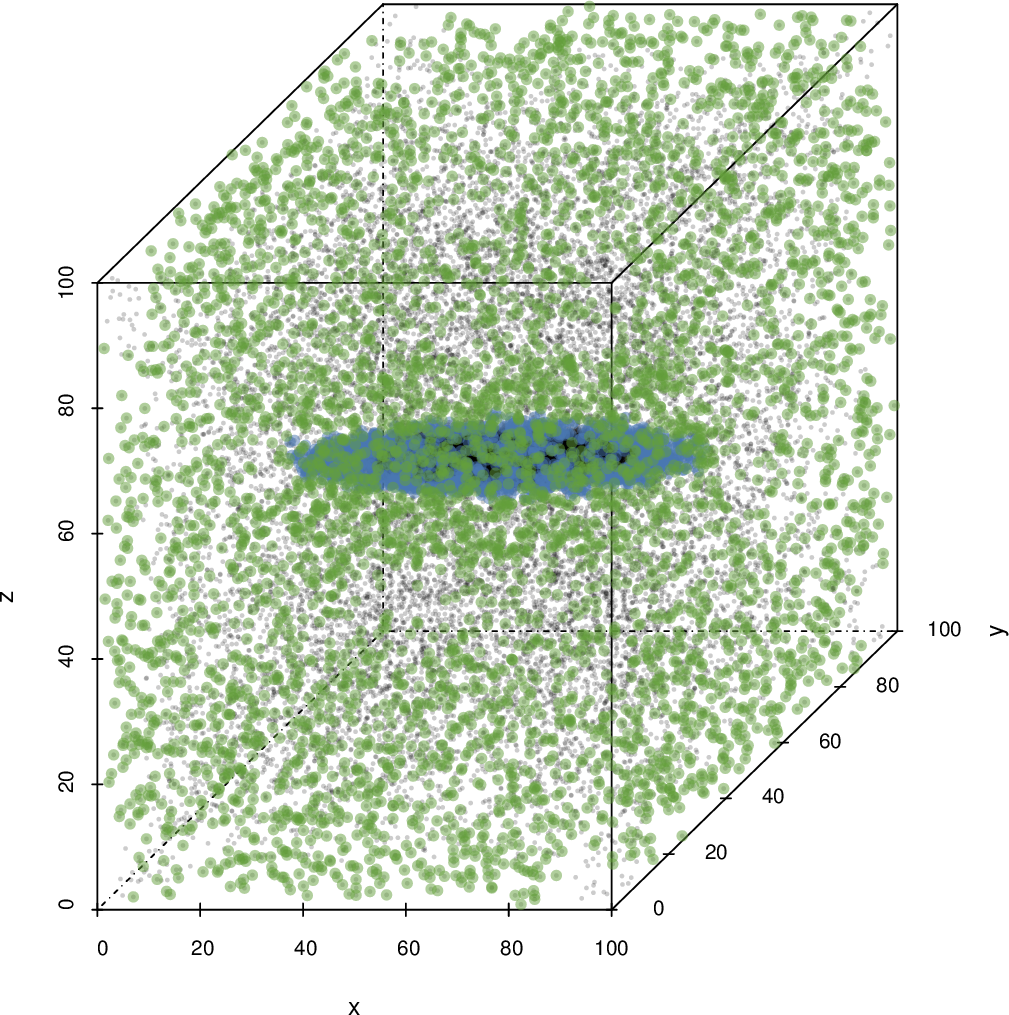
\includegraphics[keepaspectratio=true, width=\textwidth, height=0.23\textheight]{discussion/img/baakman_4_60000_anisotropy.png}
				\caption{Dataset \baakmanFour}
				\label{fig:discussion:anisotropy:baakman4}
			\end{subfigure}		
			\begin{subfigure}{0.23\textwidth}
				\centering
				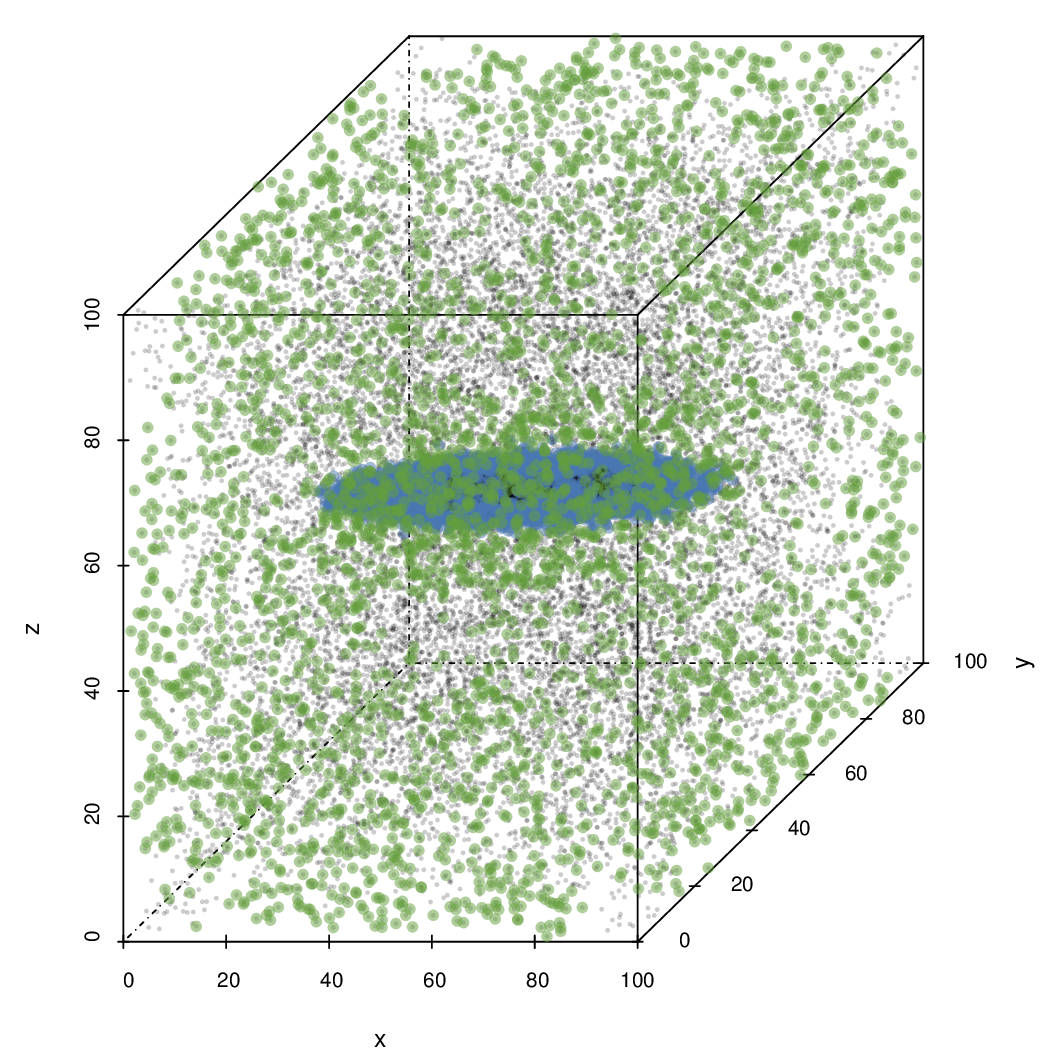
\includegraphics[keepaspectratio=true, width=\textwidth, height=0.23\textheight]{discussion/img/baakman_5_60000_anisotropy.png}
				\caption{Dataset \baakmanFive}
				\label{fig:discussion:anisotropy:baakman5}
			\end{subfigure}			
			\caption{Scatter plot of the data sets
				\subref{fig:discussion:anisotropy:ferdosi1} \ferdosiOne, %
				\subref{fig:discussion:anisotropy:baakman1} \baakmanOne, %
				\subref{fig:discussion:anisotropy:baakman4} \baakmanFour, and %
				\subref{fig:discussion:anisotropy:baakman5} \baakmanFive. %
				The points whose anisotropy lies in the \nth{90} percentile are shown larger and in the color of the component they were drawn from.}
			\label{fig:discussion:anisotropy:singleSphere}
		\end{figure}
		%	
		To that end plot \cref{fig:discussion:anisotropy:singleSphere} shows the datasets with a single Gaussian with points whose anisotropy lies in the \nth{90} percentile emphasized. 
			% Ferdosi 2 & Baakman 2
			In this figure hardly any difference is visible between \cref{fig:discussion:anisotropy:ferdosi1,fig:discussion:anisotropy:baakman1}. 
				% Very few points from Gaussian comonent
				Although it is hardly visible in the plots \SI{5.180481283422460e-01}{\percent} and \SI{1.174799465240642e+01}{\percent} of the emphasized points are sampled from the Gaussian component of dataset \ferdosiOne and \baakmanOne, respectively. Which illustrates that the kernels in dataset \baakmanOne are influenced by the anisotropy of the Gaussian component of that dataset.
				% Shell of points sampled from the noise around the Gaussian comonent
				Furthermore a shall op points sampled from the noise seems to surround the Gaussian component, it is quite likely that the shape of the kernel of these points is influenced by the Gaussian component. 
				% Explanation
				We expect that nearer to the mean of the Gaussian component fewer kernels are influenced by its anisotropy as the physical density of points is quite high in that area. Consequently the volume of the local neighborhood is quite small, and is therefore not representative of the shape of the Gaussian component. 

			% Baakman 4
			In dataset \baakmanFour and \baakmanFive the anisotropy of the kernels of the points sampled from the

			% Baakman 5

		% Some general conclusion
		
		% Multi Sphere

	% Kernel is sensitive to spurious structure in the data

% Highest anisotropy of noise component 
	% Kernel 'catches' spurious structures in noise -> increase K.

% Denser component -> higher anisotropy of kernels
% AND Higher anistropy in component -> higer anisotropy in associated kernels
% AND Denser comonent -> lower MSE
	% Introduce the dataset A1 and A2, same anisotropy different density, what do we observe, what does it say about this correlation.

% Lack of difference in anisotropy between F3 and B3 in orange (‘Trivariate Gaussian 3’) component. 

% Some conclusion

	\begin{figure}
		\centering
		\begin{subfigure}{0.23\textwidth}
			\centering
			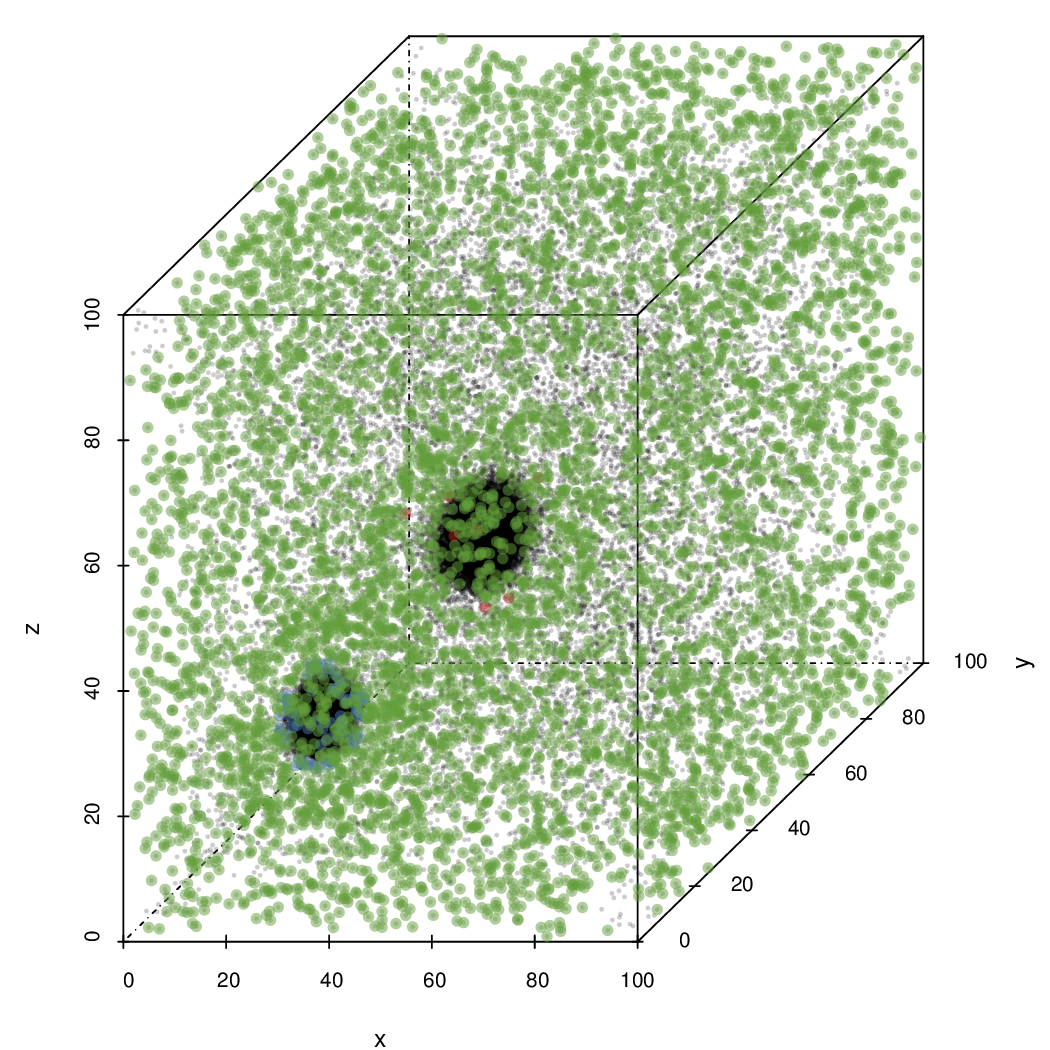
\includegraphics[keepaspectratio=true, width=\textwidth, height=0.23\textheight]{discussion/img/ferdosi_2_60000_anisotropy.png}
			\caption{Dataset \ferdosiTwo}
			\label{fig:discussion:anisotropy:ferdosi2}
		\end{subfigure}
		\begin{subfigure}{0.23\textwidth}
			\centering
			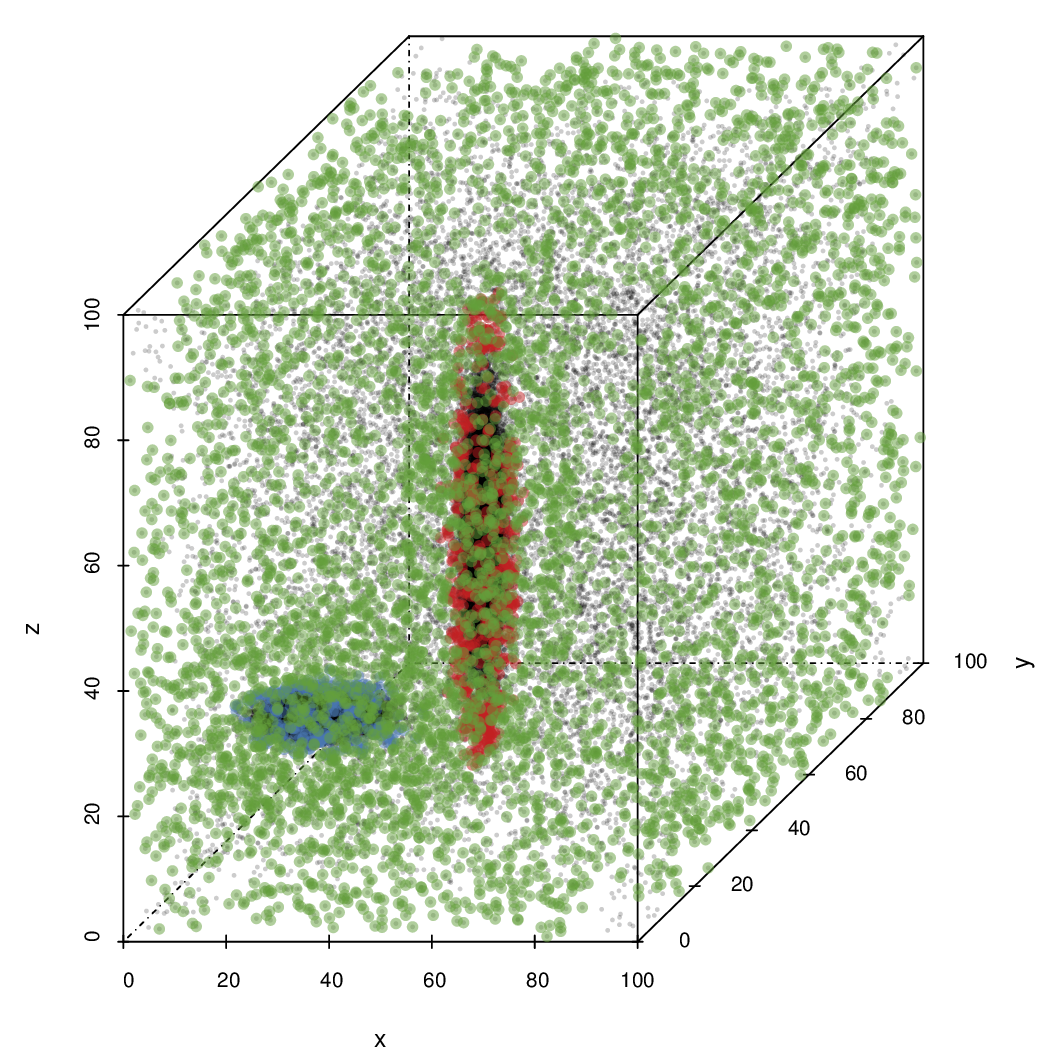
\includegraphics[keepaspectratio=true, width=\textwidth, height=0.23\textheight]{discussion/img/baakman_2_60000_anisotropy.png}
			\caption{Dataset \baakmanTwo}
			\label{fig:discussion:anisotropy:baakman2}
		\end{subfigure}	
		\begin{subfigure}{0.23\textwidth}
			\centering
			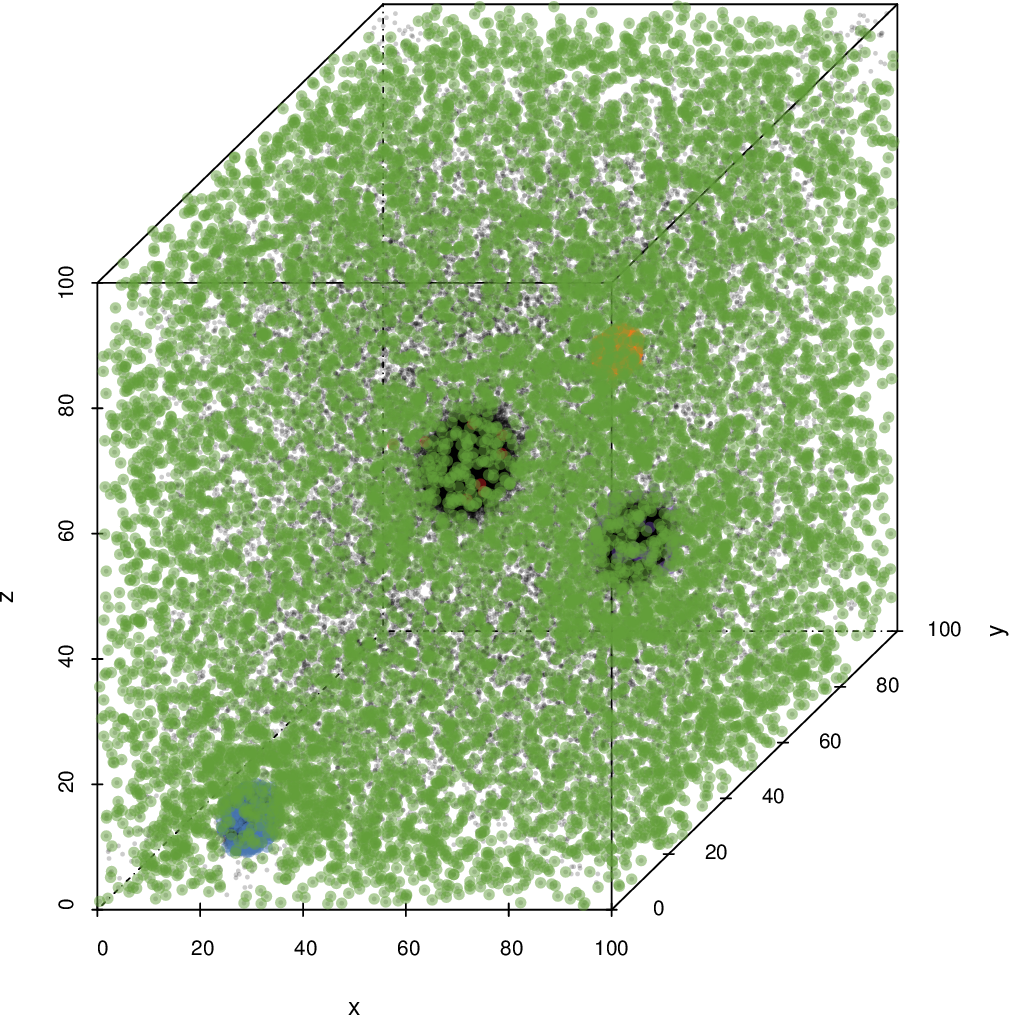
\includegraphics[keepaspectratio=true, width=\textwidth, height=0.23\textheight]{discussion/img/ferdosi_3_120000_anisotropy.png}
			\caption{Dataset \ferdosiThree}
			\label{fig:discussion:anisotropy:ferdosi3}
		\end{subfigure}		
		\begin{subfigure}{0.23\textwidth}
			\centering
			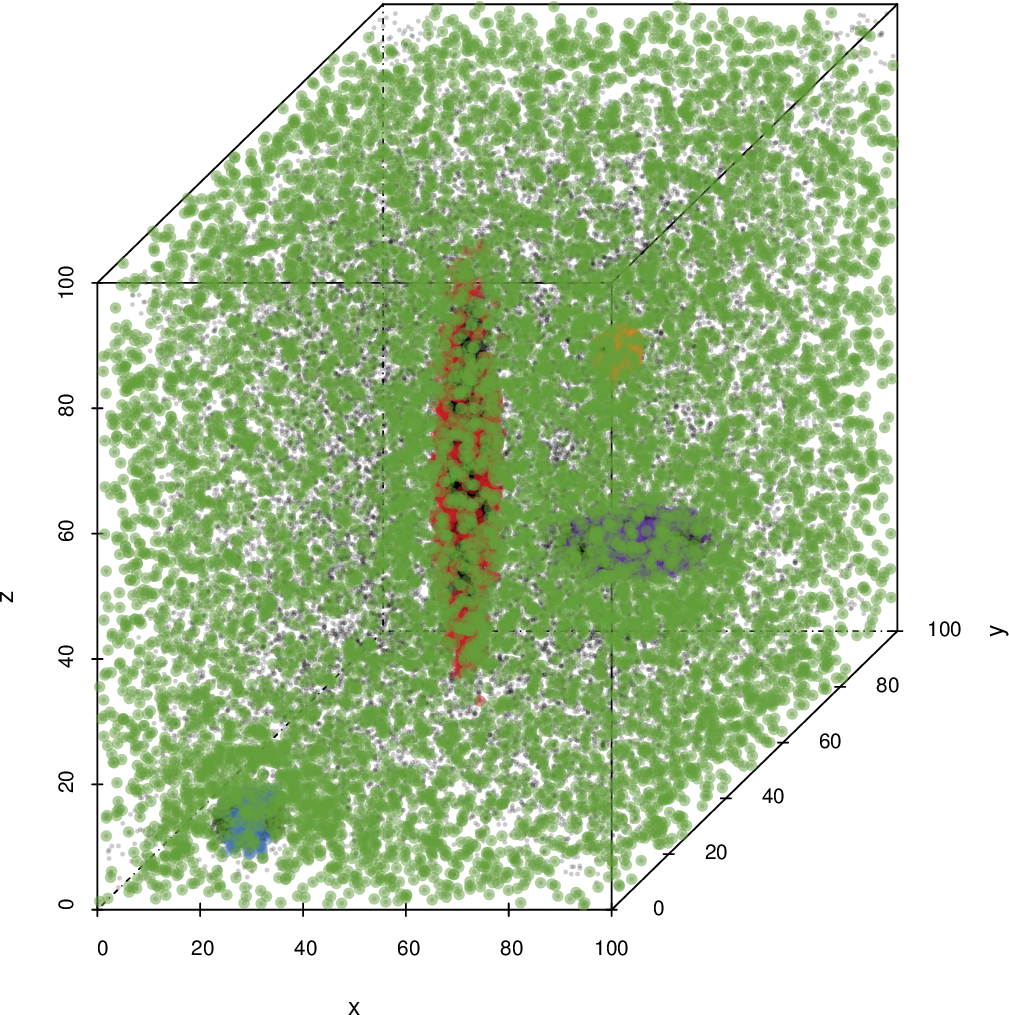
\includegraphics[keepaspectratio=true, width=\textwidth, height=0.23\textheight]{discussion/img/baakman_3_60000_anisotropy.png}
			\caption{Dataset \baakmanThree}
			\label{fig:discussion:anisotropy:baakman3}
		\end{subfigure}			
		\caption{Scatter plot of datasets
			\subref{fig:discussion:anisotropy:ferdosi2} \ferdosiTwo, %
			\subref{fig:discussion:anisotropy:baakman2} \baakmanTwo, %
			\subref{fig:discussion:anisotropy:ferdosi3} \ferdosiThree, and %
			\subref{fig:discussion:anisotropy:baakman3} \baakmanThree. %
			The points that have an anisotropy in the \nth{90} percentile are shown larger and in the color of the component they were drawn from.}
		\label{fig:discussion:anisotropy:multisphere}
	\end{figure}	